\section{Reproducible computations and numerical illustrations}
\label{sec:computations}

\subsection{What the checks establish}

The package separates three different forms of evidence.
The general theorems are proved in the preceding sections.
Exact finite checks verify rational identities or enclose particular
numbers using a proved remainder bound. Floating-point computations
check conventions and illustrate asymptotic behavior. The last category
is not used to certify equality, a zero count, or a decimal enclosure.

The harmonic verifier uses two independent exact constructions through
order thirty. One differentiates the kernel in the form
\[
 K^{(j)}(t)=
 \frac{\sqrt y}{(1+y)^{j+1}}
 \{P_j(y)\log(1+y)+Q_j(y)\},\qquad y=e^{-2t}.
\]
The other constructs $\sec z$ and
$\sec z\log\sec z$ by rational formal power-series operations.
The resulting rational and $\log2$ coefficients agree at all thirty-one
nonpositive integer arguments. The same program checks the polynomial
in the proof of $K''>0$, the rational constant $181/27$, and the
right-half-plane tail bound.

The diagonal verifier compares the Stirling expression with the
independently derived quadratic recurrence in $\mathbb Q[L]$
through $n=40$. It also checks the inverse generating equation
through degree forty after a rational formal specialization.
A positive-series enclosure of $\log2$, followed by rational interval
Horner evaluation, certifies the velocity signs for $2\le n\le40$.
The separate quantitative experiment extends exact sign enclosures
to $50\le n\le200$ and compares them with the conjectured singularity
asymptotic. Its analytic continuation and asymptotic comparisons remain
numerical diagnostics.

The barrier verifier checks ten exact symbolic identities, including
the critical-point factorization, the cubic discriminant, and the displayed
inverse-index coefficients. For $n=2,3,4,5,10,25,100$ it also isolates
the optimizer and cutoff by exact rational interval arithmetic.
The exponential evaluator reduces its argument to $[0,1]$,
uses a Taylor polynomial with the explicit tail bound
$2/(M+1)!$, and then applies outward-rounded inversion and repeated
squaring. Thus the recorded decimal endpoints are consequences of
rational comparisons, rather than the output of a floating-point
root finder.

\subsection{Harmonic zeros and the two asymptotic scales}

Table~\ref{tab:harmonic-zeros} lists diagnostic roots from the positive
Mellin-moment ratio. The first three were also substituted into
independent differentiated-kernel Mellin integrals.
Those checks do not share the digamma representation.
At forty-five working decimal digits, the three independent absolute
residuals are approximately $2.1\times10^{-43}$,
$1.1\times10^{-31}$, and $1.2\times10^{-25}$.
Working precision is not a guarantee of correct output digits, and
these values are not presented as certified intervals.

\begin{table}[htbp]
\centering
\begin{tabular}{@{}r r r@{}}
\toprule
$m$ & Approximate $\sigma_m$ & Approximate $\varepsilon_m$\\
\midrule
1   & $-2.151826895870$    & $0.848173104130$\\
2   & $-4.358674064874$    & $0.641325935126$\\
3   & $-6.454482934804$    & $0.545517065196$\\
5   & $-10.548589016994$   & $0.451410983006$\\
10  & $-20.640881124485$   & $0.359118875515$\\
50  & $-100.764467222239$  & $0.235532777761$\\
500 & $-1000.845421933140$ & $0.154578066860$\\
\bottomrule
\end{tabular}
\caption{Numerical illustrations of the proved real-zero classification.
The decimals are diagnostic approximations.}
\label{tab:harmonic-zeros}
\end{table}

\begin{figure}[htbp]
\centering
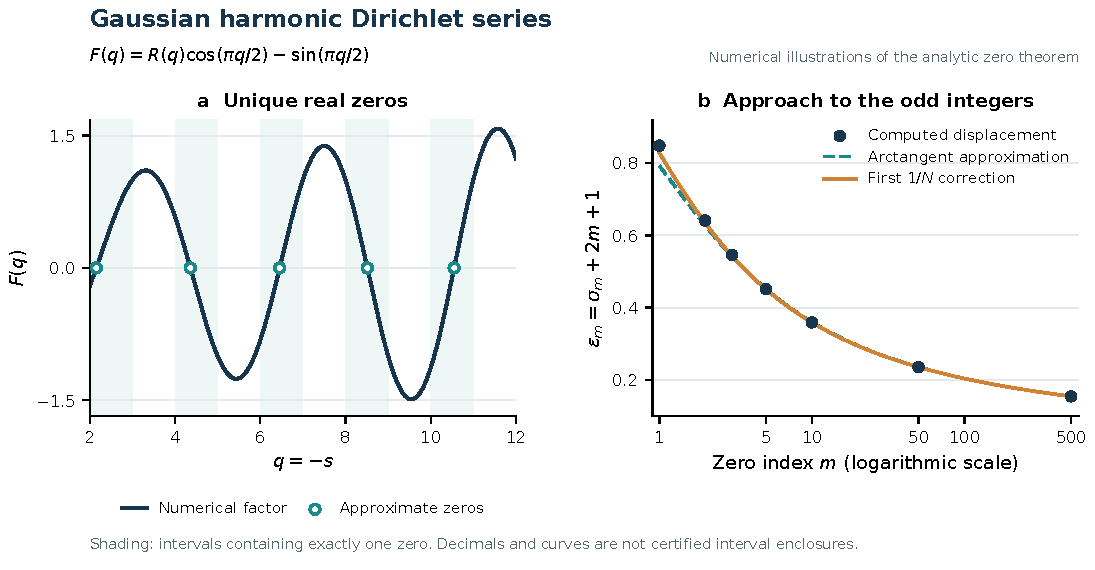
\includegraphics[width=\textwidth]{figures/harmonic_order_zeros.pdf}
\caption{The normalized Fourier factor and the real-zero displacement.
Zeros of $R(q)\cos(\pi q/2)-\sin(\pi q/2)$ give the real zeros of
$S(-q)$ because its omitted prefactor is positive.
The displacement plot compares numerical roots with the arctangent
term and its first $1/N$ correction. These curves illustrate
Theorems~\ref{sorder:thm:all-real-zeros}
and \ref{sorder:thm:zero-asymptotic}; they are not their proofs.}
\label{fig:harmonic}
\end{figure}

The first inverse-index correction need not improve an approximation
at every small index. For example, at $m=5$ the leading arctangent
term happens to be unusually close, and its next term overshoots.
The theorem concerns controlled errors as $m\to\infty$ and does not
assert a globally enveloping expansion. The distinction between the
inverse-logarithmic series and the smaller $1/N$ sectors is also
essential: retaining more logarithmic powers alone cannot resolve
an algebraically small correction in $N$.

\subsection{Certified sample cutoffs}

The cutoff enclosures in Table~\ref{tab:cutoffs} are exact.
The old fixed-coefficient cutoffs in its last column are rounded
diagnostics for comparison. In particular, the new coefficient can
reduce the compact interval remaining for a separate zero count.
That improvement does not itself supply signs on the compact interval.

\begin{table}[htbp]
\centering
\small
\begin{tabular}{@{}r l r@{}}
\toprule
$n$ & Certified enclosure for $B_n$ &
Fixed $\lambda=e^{-n}$ cutoff\\
\midrule
2 & $[1.47580064163065338930,\;1.47580064163065338931]$
  & $1.5102804080$\\
3 & $[2.27333271490894820528,\;2.27333271490894820529]$
  & $2.3431706385$\\
4 & $[3.57479611518613398335,\;3.57479611518613398336]$
  & $3.6783274602$\\
5 & $[5.69074542139040729581,\;5.69074542139040729582]$
  & $5.8264887639$\\
10 & $[63.21469931898564283555,\;63.21469931898564283556]$
  & $63.5050628049$\\
\bottomrule
\end{tabular}
\caption{Exact sample enclosures for the least uniform cutoff.
Full optimizer, coefficient, and logarithmic-cutoff intervals are
recorded in the accompanying JSON certificate.}
\label{tab:cutoffs}
\end{table}

\begin{figure}[htbp]
\centering
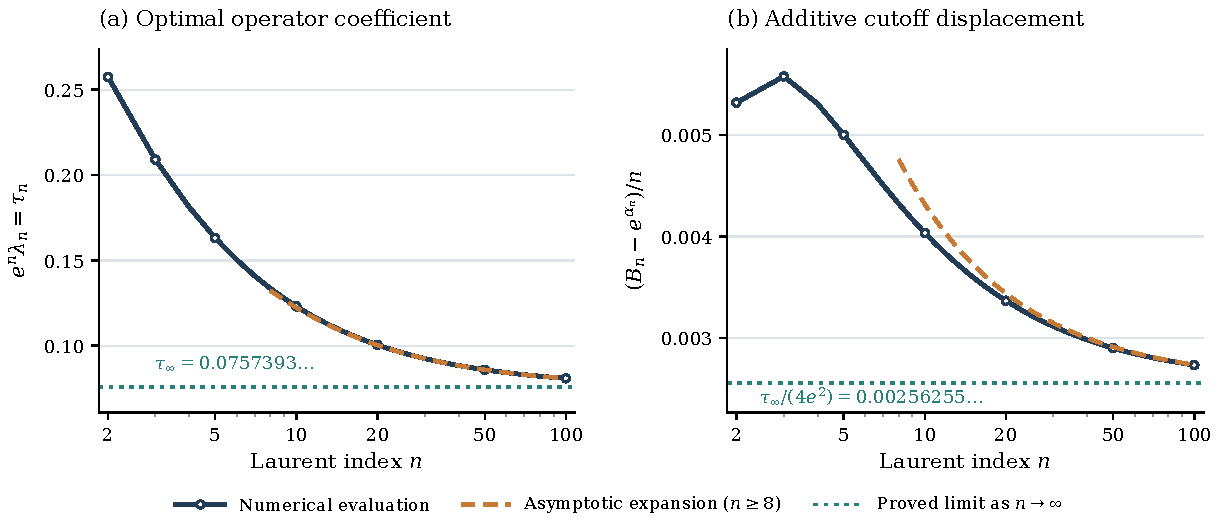
\includegraphics[width=\textwidth]{figures/optimal_barrier_parameters.pdf}
\caption{Optimal exterior-barrier parameters. Navy curves show numerical
evaluations of the proved defining formulas; teal dotted lines show
the limiting constants. Orange dashed curves, displayed for $n\ge8$,
use two inverse-index corrections for $\tau_n$ and the first correction
for the normalized cutoff displacement. Numerical evaluation illustrates
the analytic theorems; exact sample enclosures are recorded separately.}
\label{fig:barrier}
\end{figure}

For the figure, the difference $B_n-e^{\alpha_n}$ is evaluated as
$e^{\alpha_n}\operatorname{expm1}(\eta_n-\alpha_n)$ at high precision.
Subtracting the two large exponentials directly would obscure the
small displacement and can produce a misleading numerical comparison.

\subsection{Replay and build instructions}

The archive contains the complete expanded \nolinkurl{article.tex},
the modular section sources, the compiled PDF, the data records,
and all verification and plotting scripts.
The standard-library exact checks and the symbolic/interval checks
have separate entry points:
\begin{minipage}{\textwidth}
\begin{verbatim}
python3 code/verify_diagonal.py
python3 code/verify_gaussian_order.py --output data/gaussian_exact.json
python3 code/verify_optimal_barrier.py \
  --output data/optimal_barrier_verification.json
\end{verbatim}
\end{minipage}
The full numerical and quantitative commands, package requirements,
and figure regeneration steps are in \nolinkurl{README.md}.
The optional numerical routines use mpmath, and the scientific figures
use Matplotlib and SciPy. A requirements file records the environment
used for the delivered run.

To regenerate the expanded TeX and PDF from the modular sources:
\begin{verbatim}
python3 code/assemble_article.py
latexmk -pdf -interaction=nonstopmode -halt-on-error article.tex
\end{verbatim}
The distributed PDF was built from the same expanded source and
visually checked. The build and verification records are included.
The source snapshot identifies the baseline for later integration;
the package does not modify the remote repository.
